\documentclass{standalone}
\usepackage{tikz}
\usetikzlibrary{shapes,arrows,calc,positioning,backgrounds,plotmarks,plothandlers,fit}


\begin{document}

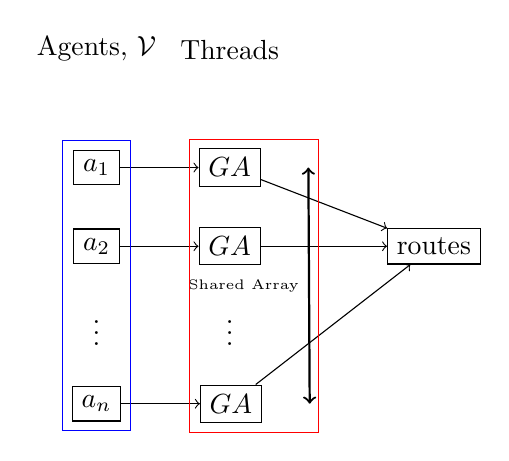
\begin{tikzpicture}
  \node[draw,rectangle] (A1) {$a_{1}$};
  \node[draw,rectangle, below of=A1] (A2) {$a_{2}$};
  \node[below of=A2] (ellipses) {$\vdots$};
  \node[draw,rectangle, below of=ellipses] (An) {$a_{n}$};

  \node[draw,rectangle, right= of A1] (GA1) {$GA$};
  \node[draw,rectangle, right= of A2] (GA2) {$GA$};
  \node[below of=GA2] (ellipses2) {$\vdots$};
  \node[draw,rectangle, right= of An] (GAn) {$GA$};

  \coordinate[right of = GA1] (rGA1);
  \coordinate[right of = GA2] (rGA2);
  \coordinate[right of = GAn] (rGAn);

  \node[draw, rectangle, right= of rGA2] (result) {routes};

  \node[above = of GA1] (lthreads) {Threads};
  \node[above = of A1] (lagents) {Agents, $\mathcal{V}$};


  \draw[->] (A1) -> (GA1);
  \draw[->] (A2) -> (GA2);
  \draw[->] (An) -> (GAn);

  \draw[->] (GA1) -> (result);
  \draw[->] (GA2) -> (result);
  \draw[->] (GAn) -> (result);


  \draw[thick,<->] (rGAn) -> node[left] {\tiny Shared Array} (rGA1);


  \node[draw=red, fit=(GA1) (GAn) (rGAn)]  {};
  \node[draw=blue, fit=(A1) (An)]  {};


\end{tikzpicture}

\end{document}
